\chapter{Interfaccia seriale}

\section{UART}

Sfruttando l’implementazione fornita dalla Digilent di un dispositivo UART (componente RS232RefComp.vhd), progettare e implementare in VHDL un sistema costituito da 2 nodi A e B collegati tra loro mediante una interfaccia seriale. Il sistema A acquisisce una stringa di 8 bit dall’utente (mediante gli switch della board di sviluppo) e la invia mediante la seriale al sistema B, che la manda in output sui led della board di sviluppo. 

\subsection{Descrizione UART}
Il dispositivo UART della Digilent è in grado di operare in modalità \textit{full duplex}, ed è formata da due componenti principali: un trasmettitore e un ricevitore.
La frame dei dati utilizzata per la trasmissione prevede due bit per marcare l'inizio e la fine del messaggio, e otto bit per i dati effettivi.


\begin{figure}[H]
    \centering
    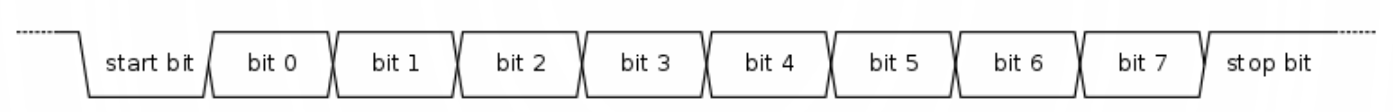
\includegraphics[width=17cm]{immagini/esercizio9/frame.png}
    \caption{Frame UART}
    \label{fig:my_label}
\end{figure}

Lo stato di inattività viene mostrato da un bit alto, in modo da poter constatare in ogni caso il corretto funzionamento del sistema senza creare ambiguità (se fosse basso non sarebbe possibile distinguere il caso di non trasmissione da quello di linea interrotta).

Il ricevitore ha il compito di prendere i dati seriali in ingresso e convertirli in parallelo. Un registro a scorrimento viene utilizzato per memorizzare i dati in ingresso sulla porta \textit{RXD}. Un controller si occupa di gestire i segnali tra i diversi componenti e genera l'uscita \textit{RDA} per notificare la fine della ricezione. Lo schema dell'automa del controller è mostrato nella figura.

\begin{figure}[H]
    \centering
    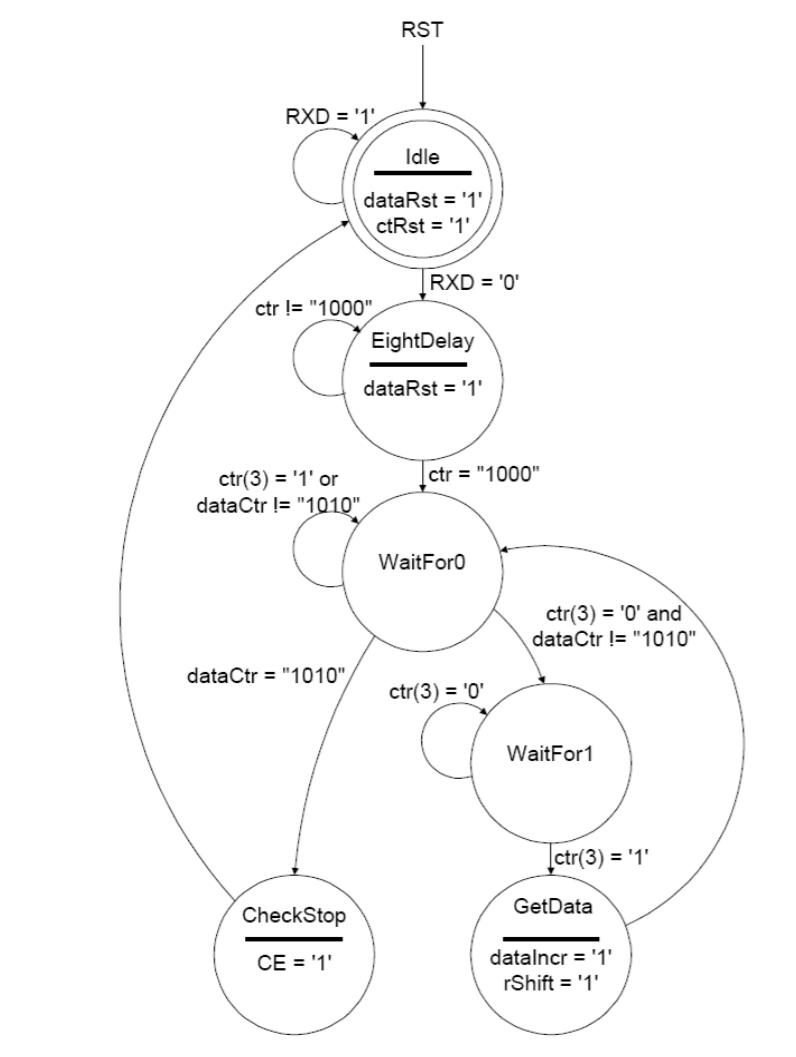
\includegraphics[width=11cm]{immagini/esercizio9/ricevitore_automa.png}
    \caption{Automa Ricevitore}
    \label{fig:my_label}
\end{figure}

Il trasmettitore ha il compito di prendere i dati paralleli in input e inviarli uno alla volta sull'uscita \textit{TXD}. Anche questo componente ha un controller che gestisce la velocità di trasmissione e il numero dei bit inviati. Lo schema dell'automa del controller è mostrato in figura. 

\begin{figure}[H]
    \centering
    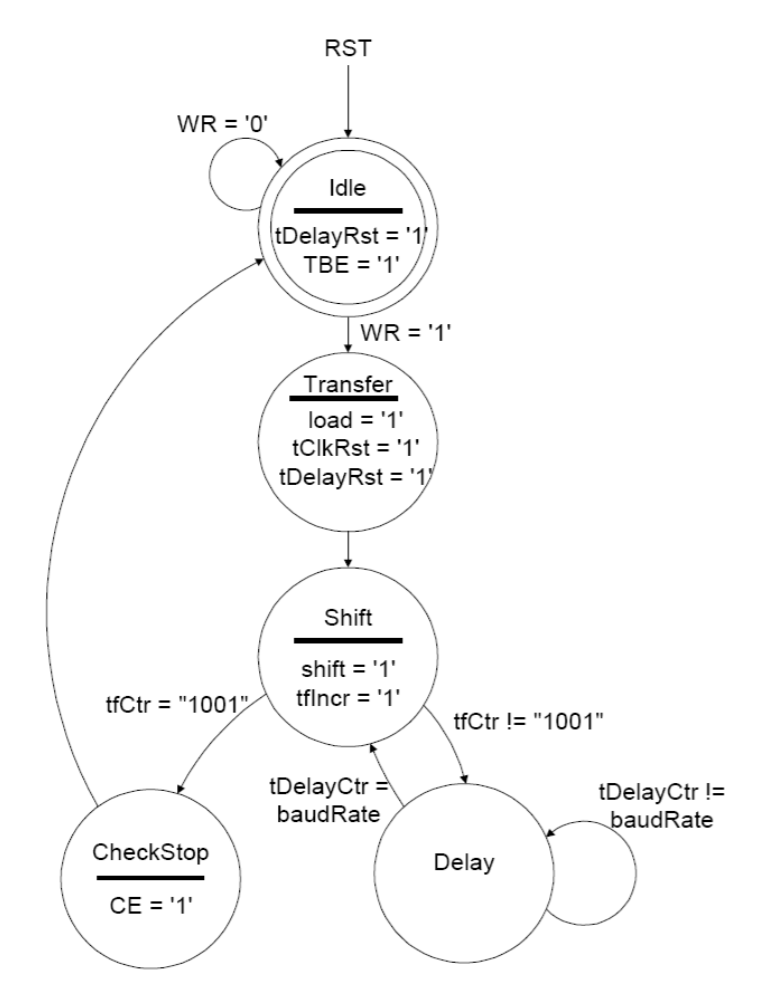
\includegraphics[width=11cm]{immagini/esercizio9/trasmettitore_automa.png}
    \caption{Automa Trasmettitore}
    \label{fig:my_label}
\end{figure}
Il ricevitore e il trasmettitore non condividono normalmente lo stesso clock, per cui viene stabilito il numero di transizioni con il \textit{baud rate}. Questo può essere calcolato come:
\begin{equation*}
    \frac{frequenza\;clock}{baud}
\end{equation*}

dove il baud è uguale a 115200. La frequenza del ricevitore, che deve sovra-campionare la linea in modo da essere 16 volte più veloce del trasmettitore, può essere ottenuta con il \textit{baud divide}, calcolabile come:
\begin{equation*}
    \frac{baud\;rate\;clock}{16}
\end{equation*}

\subsection{Architettura}

La soluzione è stata realizzata seguendo un approccio strutturale, partendo dalla creazione dei due sistemi separati, A e B, e procedendo con l'interconnessione di essi. 

Il sistema A è composto da:
\begin{itemize}
    \item \textit{registro}: un flip flop che memorizza la stringa inserita dall'utente;
    \item \textit{UART}: il componente, fornitoci a priori, costituisce in un'interfaccia per la trasmissione del dato tra i due sistemi;
    \item \textit{rete di controllo}: regola che la trasmissione dei dati avvenga in modo corretto.
\end{itemize}

Il sistema B, invece, è composto da:
\begin{itemize}
    \item \textit{registro}: un flip flop che memorizza la stringa ricevuta dal sistema A, che esce dal ricevitore UART;
    \item \textit{UART}: il componente, fornitoci a priori, costituisce in un'interfaccia per la ricezione della stringa;
    \item \textit{rete di controllo}: regola che la trasmissione e l'output dei dati avvenga in modo corretto.
\end{itemize}

Le interconnessioni tra i due sistemi sono visibili nella seguente architettura: 
\begin{figure}[H]
    \centering
    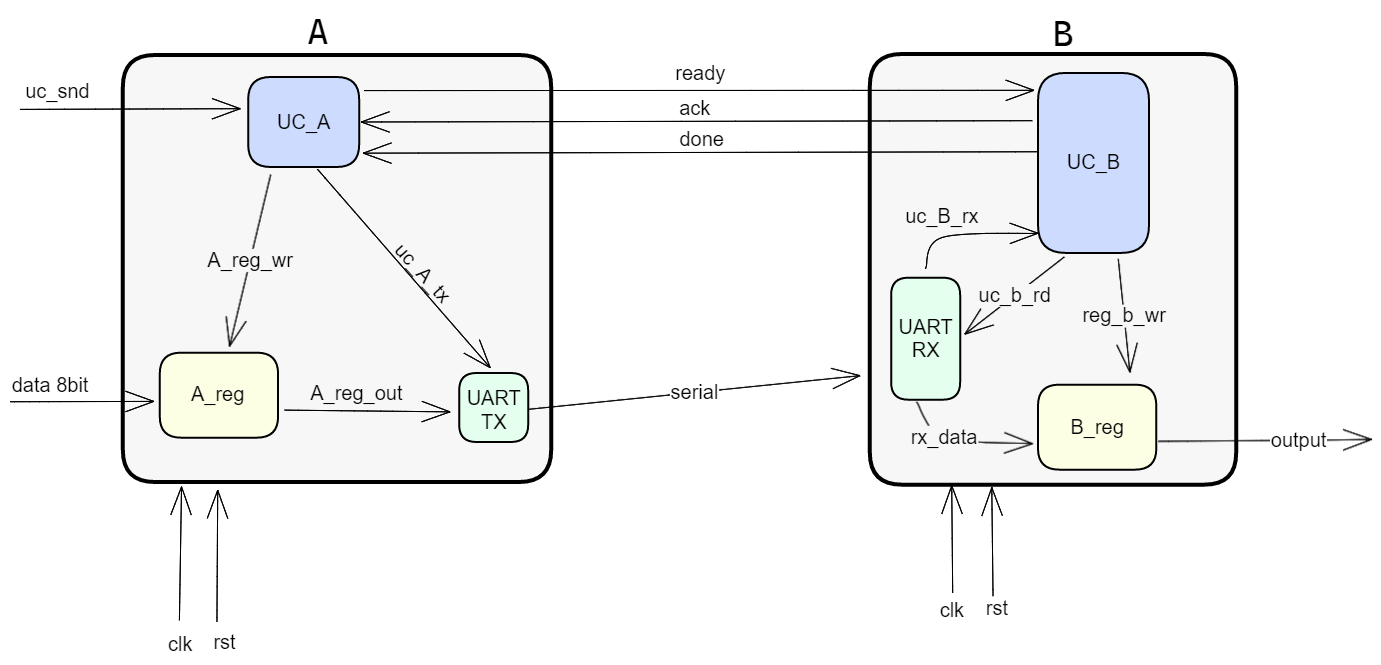
\includegraphics[width=18cm]{immagini/esercizio9/schema_9.1.png}
    \caption{Schema Interfaccia Seriale}
    \label{fig:my_label}
\end{figure}
I componenti registro e UART sono basati su quelli descritti nelle sezioni precedenti.
Le reti di controllo di A e B si occupano di gestire non solo i componenti del proprio sistema, ma comunicano tra loro in modo da sincronizzare l'inizio e la fine della trasmissione.
Anche se non richiesto dalla traccia, è stata inserita una logica di handshaking a 3 passaggi (three way handshaking) in modo da assicurarsi non solo che tutti e due i dispositivi siano pronti alla trasmissione, ma che il dato arrivi a destinazione nella sua interezza. Questo è particolarmente importante dato che il ricevitore deve essere già pronto quando il trasmettitore inizia a inviare. 
Questa aggiunta è stata utile anche per sperimentare metodi di controllo più avanzati della seriale, che sono stati poi utilizzati nell'esercizio a scelta finale, ed è stata fatta in questo esercizio e non nel successivo (9.2) per iniziare a testarlo con un sistema meno complesso.

Nell'automa di A ci sono tre condizioni che bloccano il sistema con un auto-anello: innanzitutto deve arrivare il segnale di \textit{send} dall'esterno, per iniziare il processo di trasmissione, in seguito il sistema alza il segnale \textit{ready} e aspetta l'ack di B. Una volta arrivato l'ack inizia la trasmissione con la UART, alzando il segnale uc\_A\_tx, e si aspetta che B riceva l'intero messaggio e alzi il segnale \textit{done}.


Nell'automa di B ci sono due auto-anelli: il primo aspetta che A alzi il segnale di \textit{ready}, in modo da poter mandare l'\textit{ack} e in seguito si aspetta che la periferica UART alzi il segnale \textit{uc\_B\_rx}, detto anche RDA. Questo segnale indica la fine della ricezione del messaggio, per cui sarà possibile scrivere il risultato nel registro e confermare la fine della trasmissione alzando il \textit{done}.

Di seguito è possibile osservare la stesura degli automi dei singoli sistemi: 

\begin{figure}[H]
    \centering
    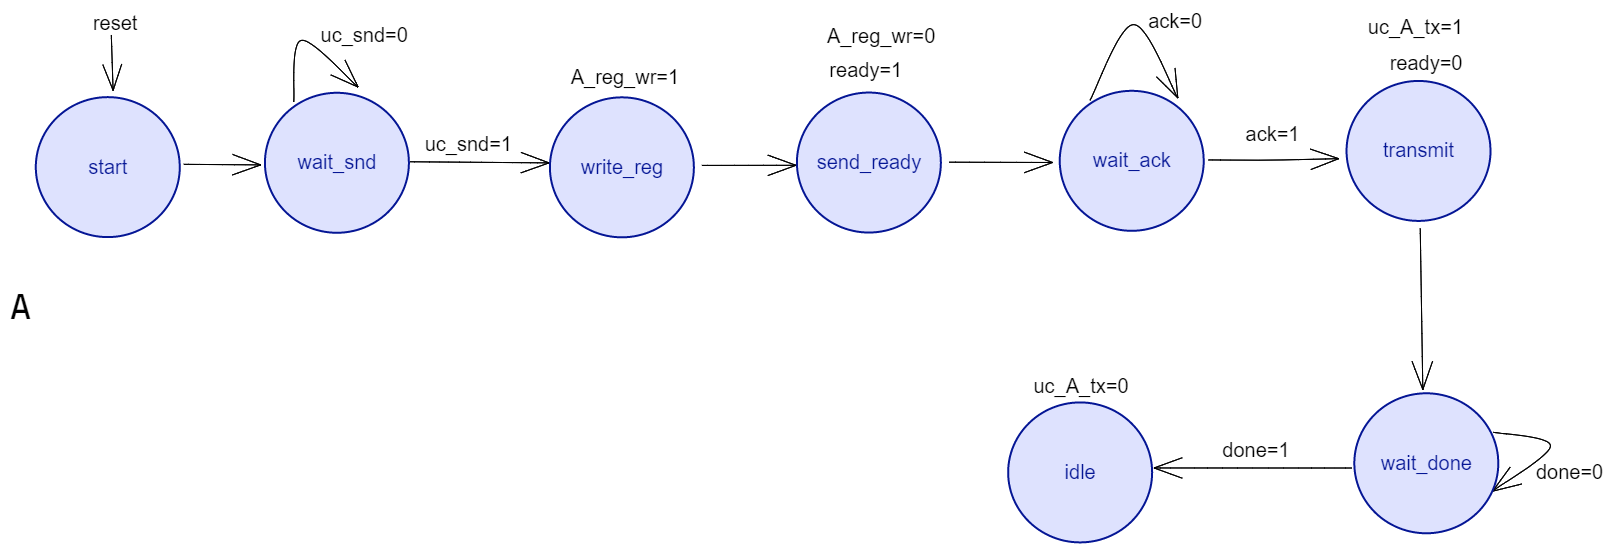
\includegraphics[width=17cm]{immagini/esercizio9/automaA_9.1.png}
    \caption{Automa A}
\end{figure}

\begin{figure}[H]
    \centering
    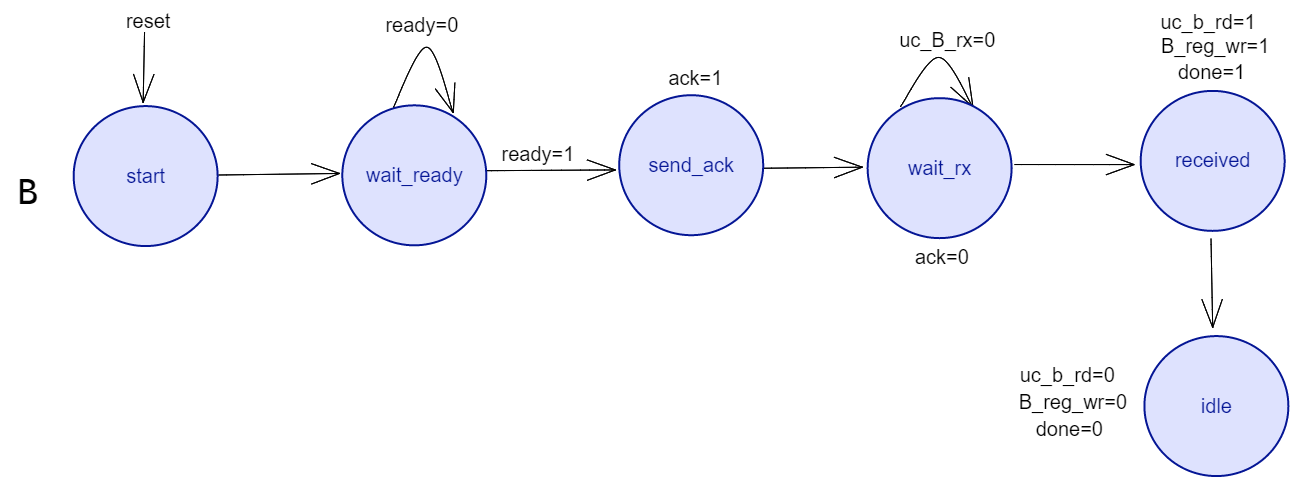
\includegraphics[width=17cm]{immagini/esercizio9/automaB_9.1.png}
    \caption{Automa B}
\end{figure}


Di seguito è mostrato il codice dei sistemi A e B.
N.B.: per semplicità è stato omesso il codice della UART.

\begin{lstlisting} [language=VHDL, caption=Registro]
library IEEE;
use IEEE.STD_LOGIC_1164.ALL;

entity reg is
    Port (
        din: in std_logic_vector(7 downto 0);
        clk, rst, wr: in std_logic;
        dout: out std_logic_vector(7 downto 0)
       );
end reg;

architecture Behavioral of reg is
begin
    ff: process(clk)
        begin
            if rising_edge(clk) then
                if rst = '1' then
                    dout <= (others => '0');
                elsif wr = '1' then
                    dout <= din;
                end if;
            end if;
    end process ff;
end Behavioral;
\end{lstlisting}

\begin{lstlisting} [language=VHDL, caption=Rete di controllo di A]
library IEEE;
use IEEE.STD_LOGIC_1164.ALL;
use IEEE.std_logic_unsigned.all;

entity uc_a is
    port(
        clk, rst, ack, done, uc_snd: in std_logic;
        ready, uc_a_tx, reg_a_wr : out std_logic
    );
end uc_a;

architecture behavioral of uc_a is

    type state is (
        IDLE,
        START,
        WAIT_SND,
        WRITE_REG,
        SND_READY,
        WAIT_ACK,
        TRANSMIT,
        WAIT_DONE
    );
    
    signal current_state : state:= IDLE;
    signal next_state : state;
  
begin
    comb: process(current_state, ack, done, uc_snd)
    begin
        case current_state is
        
            when START =>
                ready <= '0';
                uc_a_tx <= '0';
                reg_a_wr <= '0';
                next_state<= WAIT_SND;
                
            when WAIT_SND=>
                if ( uc_snd = '1' ) then
                    next_state <= WRITE_REG;
                else
                    next_state <= WAIT_SND;
                end if;
                
            when WRITE_REG=>
                reg_a_wr <= '1';
                next_state <= SND_READY;
                
            when SND_READY=>
                reg_a_wr <= '0';
                ready <= '1';
                next_state <= WAIT_ACK;
                
            when WAIT_ACK=>
                if ( ack = '1' ) then
                    next_state <= TRANSMIT;
                else
                    next_state <= WAIT_ACK;
                end if;
                
            when TRANSMIT=>
                uc_a_tx <= '1';
                ready <= '0';
                next_state <= WAIT_DONE;
                
            when WAIT_DONE=>
                if ( done = '1' ) then
                    next_state <= IDLE;
                else
                    next_state <= WAIT_DONE;
                end if;
                
            when IDLE=>
                uc_a_tx <= '0';
                
            when others => next_state<= IDLE;
        end case;
    end process comb;

    seq: process(clk)
    begin
        if rising_edge(clk) then
            if rst='1'  then
                current_state<=START;
            else
                current_state<=next_state;
            end if;
        end if;
    end process seq;
    
end behavioral;
\end{lstlisting}

Di seguito il codice di A:
\begin{lstlisting} [language=VHDL, caption=Sistema A]
library IEEE;
use IEEE.STD_LOGIC_1164.ALL;

entity a is
 Port (
    uc_snd, clk, rst, ack, done: in std_logic;
    data : in std_logic_vector(7 downto 0);
    output, ready: out std_logic
  );
end a;

architecture Structural of a is

component UARTcomponent is
	Generic (
		--@48MHz
--		BAUD_DIVIDE_G : integer := 26; 	--115200 baud
--		BAUD_RATE_G   : integer := 417

		--@26.6MHz
		BAUD_DIVIDE_G : integer := 14; 	--115200 baud
		BAUD_RATE_G   : integer := 231
	);
	Port (	
		TXD 	: out 	std_logic  	:= '1';					-- Transmitted serial data output
		RXD 	: in  	std_logic;							-- Received serial data input
		CLK 	: in  	std_logic;							-- Clock signal
		DBIN 	: in  	std_logic_vector (7 downto 0);		-- Input parallel data to be transmitted
		DBOUT 	: out 	std_logic_vector (7 downto 0);		-- Recevived parallel data output
		RDA		: inout  std_logic;							-- Read Data Available
		TBE		: out 	std_logic 	:= '1';					-- Transfer Buffer Emty
		RD		: in  	std_logic;							-- Read Strobe
		WR		: in  	std_logic;							-- Write Strobe
		PE		: out 	std_logic;							-- Parity error		
		FE		: out 	std_logic;							-- Frame error
		OE		: out 	std_logic;							-- Overwrite error
		RST		: in  	std_logic	:= '0');				-- Reset signal
						
end component  UARTcomponent;

component uc_a is
    port(
        clk, rst, ack, done, uc_snd: in std_logic;
        ready, uc_a_tx, reg_a_wr : out std_logic
    );
end component uc_a;

component reg is
    Port (
        din: in std_logic_vector(7 downto 0);
        clk, rst, wr: in std_logic;
        dout: out std_logic_vector(7 downto 0)
       );
end component reg;

signal reg_a_wr, uc_a_tx: std_logic;
signal reg_a_out: std_logic_vector(7 downto 0);

begin

a_reg: reg port map(
    din=>data,
    clk=>clk,
    rst=>rst,
    wr=>reg_a_wr,
    dout => reg_a_out
);

cu: uc_a port map(
    clk=>clk,
    rst=>rst,
    done=>done,
    ack=>ack,
    ready=>ready,
    uc_a_tx=> uc_a_tx,
    uc_snd=> uc_snd,
    reg_a_wr=>reg_a_wr
);

uart:  UARTcomponent generic map(
    BAUD_DIVIDE_G=>26,
    BAUD_RATE_G=>417
)
port map (
    TXD => output,
    RXD => '1',
    CLK => clk,
    DBIN => reg_a_out,
    DBOUT => OPEN,
    RDA => OPEN,
    TBE => OPEN,
    RD => '0',
    WR => uc_a_tx,
    PE => OPEN,
    FE => OPEN,
    OE => OPEN,
    RST => rst
);
end Structural;
\end{lstlisting}

I componenti del sistema B sono stati implementati anch'essi tramite un'architettura "Behavioral", di seguito il codice di ognuno di essi:

N.B.: il codice del registro coincide con il codice del registro del sistema A e per semplicità è stato omesso il codice della UART.

\begin{lstlisting} [language=VHDL, caption=Rete di controllo di B]
library IEEE;
use IEEE.STD_LOGIC_1164.ALL;
use IEEE.std_logic_unsigned.all;

entity uc_b is
    port(
        clk, rst, ready,  uc_b_rx: in std_logic;
        ack, done, reg_b_wr, uc_b_rd : out std_logic
    );
end uc_b;

architecture behavioral of uc_b is
    type state is (
        START,
        WAIT_READY,
        SND_ACK,
        WAIT_RX,
        RECEIVED,
        IDLE
    );
    
    signal current_state : state:= IDLE;
    signal next_state : state;
  
begin
    comb: process(current_state, uc_b_rx, ready)
    begin
        case current_state is
            when START =>
                done <= '0';
                reg_b_wr <= '0';
                ack <= '0';
                uc_b_rd <= '0';
                next_state<= WAIT_READY;
                
            when WAIT_READY=>
                if ( ready = '1' ) then
                    next_state <= SND_ACK;
                else
                    next_state <= WAIT_READY;
                end if;
                
            when SND_ACK=>
                ack <= '1';
                next_state <= WAIT_RX;
                
            when WAIT_RX=>
                ack <= '0';
                if ( uc_b_rx = '1' ) then
                    next_state <= RECEIVED;
                else
                    next_state <= WAIT_RX;
                end if;
                
            when RECEIVED=>
               done <= '1';
               uc_b_rd <= '1';
               reg_b_wr <= '1';
               next_state <= IDLE;
               
            when IDLE=>
                reg_b_wr <= '0';
                uc_b_rd <= '0';
                next_state <= IDLE;
                
            when others => next_state<= IDLE;
        end case;
    end process comb;

    seq: process(clk)
    begin
        if rising_edge(clk) then
            if rst='1'  then
                current_state<=START;
            else
                current_state<=next_state;
            end if;
        end if;
    end process seq;
end behavioral;
\end{lstlisting}

Di seguito il codice di B:
\begin{lstlisting} [language=VHDL, caption=Sistema B]
library IEEE;
use IEEE.STD_LOGIC_1164.ALL;

entity b is
    Port (
        ready, clk, rst, din: in std_logic;
        ack, done: out std_logic;
        dout: out std_logic_vector(7 downto 0)
    );
end b;

architecture Behavioral of b is

    component UARTcomponent is
        Generic (
            --@48MHz
            --		BAUD_DIVIDE_G : integer := 26; 	--115200 baud
            --		BAUD_RATE_G   : integer := 417

            --@26.6MHz
            BAUD_DIVIDE_G : integer := 14; 	--115200 baud
            BAUD_RATE_G   : integer := 231
        );
        Port (
            TXD 	: out 	std_logic  	:= '1';					-- Transmitted serial data output
            RXD 	: in  	std_logic;							-- Received serial data input
            CLK 	: in  	std_logic;							-- Clock signal
            DBIN 	: in  	std_logic_vector (7 downto 0);		-- Input parallel data to be transmitted
            DBOUT 	: out 	std_logic_vector (7 downto 0);		-- Recevived parallel data output
            RDA		: inout  std_logic;							-- Read Data Available
            TBE		: out 	std_logic 	:= '1';					-- Transfer Buffer Emty
            RD		: in  	std_logic;							-- Read Strobe
            WR		: in  	std_logic;							-- Write Strobe
            PE		: out 	std_logic;							-- Parity error		
            FE		: out 	std_logic;							-- Frame error
            OE		: out 	std_logic;							-- Overwrite error
            RST		: in  	std_logic	:= '0');				-- Reset signal

    end component  UARTcomponent;

    component uc_b is
        port(
            clk, rst, ready,  uc_b_rx: in std_logic;
            ack, done, reg_b_wr, uc_b_rd : out std_logic
        );
    end component uc_b;

    component reg is
        Port (
            din: in std_logic_vector(7 downto 0);
            clk, rst, wr: in std_logic;
            dout: out std_logic_vector(7 downto 0)
        );
    end component reg;

    signal rx_data: std_logic_vector(7 downto 0);
    signal reg_b_wr, uc_b_rd, uc_b_rx: std_logic;

begin
    b_reg: reg port map(
            din=>rx_data,
            clk=>clk,
            rst=>rst,
            wr=>reg_b_wr,
            dout => dout
        );

    cu: uc_b port map(
            clk=>clk,
            rst=>rst,
            done=>done,
            ack=>ack,
            ready=>ready,
            uc_b_rx => uc_b_rx,
            reg_b_wr => reg_b_wr,
            uc_b_rd=>uc_b_rd
        );

    uart:  UARTcomponent generic map(
            BAUD_DIVIDE_G=>26,
            BAUD_RATE_G=>417
        )
        port map (
            TXD => OPEN,
            RXD => din,
            CLK => clk,
            DBIN => "00000000",
            DBOUT => rx_data,
            RDA => uc_b_rx,
            TBE => OPEN,
            RD => uc_b_rd,
            WR => '0',
            PE => OPEN,
            FE => OPEN,
            OE => OPEN,
            RST => rst
        );
        
end Behavioral;
\end{lstlisting}

Infine, è possibile osservare il codice dell'intero sistema AB:
\begin{lstlisting} [language=VHDL, caption=Sistema AB]
library IEEE;
use IEEE.STD_LOGIC_1164.ALL;

entity ab is
 Port ( 
    snd, clk, rst: in std_logic;
    din : in std_logic_vector(7 downto 0);
    dout : out std_logic_vector(7 downto 0)
 );
end ab;

architecture Behavioral of ab is

component a is
 Port (
    uc_snd, clk, rst, ack, done: in std_logic;
    data : in std_logic_vector(7 downto 0);
    output, ready: out std_logic
  );
end component a;

component b is
    Port (
        ready, clk, rst, din: in std_logic;
        ack, done: out std_logic;
        dout: out std_logic_vector(7 downto 0)
    );
end component b;

signal s_ready, s_ack, s_done, s_serial_out: std_logic;

begin

UnitA: a port map(
    clk=>clk,
    rst=>rst,
    ready=>s_ready,
    ack=>s_ack,
    done=>s_done,
    output=>s_serial_out,
    
    uc_snd=>snd,
    data=>din
);

UnitB: b port map(
    clk=>clk,
    rst=>rst,
    ready=>s_ready,
    ack=>s_ack,
    done=>s_done,
    din=>s_serial_out,
    dout=>dout
);

end Behavioral;

\end{lstlisting}

\subsection{Simulazione}
Per una maggiore sicurezza si è scelto di testare prima il sistema A singolarmente e poi di effettuare la simulazione dell'intero sistema di Interfaccia Seriale.
\paragraph{Testbench}

\begin{lstlisting} [language=VHDL, caption=Testing sistema A]
library IEEE;
use IEEE.STD_LOGIC_1164.ALL;

entity a_tb is
end a_tb;

architecture Behavioral of a_tb is

    component A is
        Port (
            uc_snd, clk, rst, ack, done: in std_logic;
            data : in std_logic_vector(7 downto 0);
            output, ready: out std_logic
        );
    end component A;

    component UARTcomponent is
        Generic (
            --@48MHz
            --		BAUD_DIVIDE_G : integer := 26; 	--115200 baud
            --		BAUD_RATE_G   : integer := 417

            --@26.6MHz
            BAUD_DIVIDE_G : integer := 14; 	--115200 baud
            BAUD_RATE_G   : integer := 231
        );
        Port (
            TXD 	: out 	std_logic  	:= '1';					-- Transmitted serial data output
            RXD 	: in  	std_logic;							-- Received serial data input
            CLK 	: in  	std_logic;							-- Clock signal
            DBIN 	: in  	std_logic_vector (7 downto 0);		-- Input parallel data to be transmitted
            DBOUT 	: out 	std_logic_vector (7 downto 0);		-- Recevived parallel data output
            RDA		: inout  std_logic;							-- Read Data Available
            TBE		: out 	std_logic 	:= '1';					-- Transfer Buffer Emty
            RD		: in  	std_logic;							-- Read Strobe
            WR		: in  	std_logic;							-- Write Strobe
            PE		: out 	std_logic;							-- Parity error		
            FE		    : out 	std_logic;							-- Frame error
            OE		: out 	std_logic;							-- Overwrite error
            RST		: in  	std_logic	:= '0'
        );				-- Reset signal

    end component UARTcomponent;

    signal s_clk, s_uc_snd, s_ack, s_rst, s_ready, s_done, s_rda, s_rd: std_logic := '0';
    signal s_out_serial: std_logic := '1';
    signal s_data, s_out: std_logic_vector (7 downto 0);
    constant clk_period: time := 20ps;

begin
    uut: A port map(
            uc_snd=>s_uc_snd,
            clk=>s_clk,
            ack=>s_ack,
            rst=>s_rst,
            done => s_done,
            ready=>s_ready,
            data=>s_data,
            output => s_out_serial
        );

    rx:  UARTcomponent generic map(
            BAUD_DIVIDE_G=>26,
            BAUD_RATE_G=>417
        )
        port map (
            TXD => OPEN,
            RXD => s_out_serial,
            CLK => s_clk,
            DBIN => "00000000",
            DBOUT => s_out,
            RDA => s_rda,
            TBE => OPEN,
            RD => s_rd,
            WR => '0',
            PE => OPEN,
            FE => OPEN,
            OE => OPEN,
            RST => s_rst
        );

    tb: process
    begin
        wait for 100ns;
        s_rst <='1';
        wait for clk_period;
        s_rst <='0';
        wait for clk_period;
        s_data <= "11111111";
        wait for clk_period;
        s_uc_snd <= '1';
        wait for clk_period;
        s_uc_snd <= '0';

        wait until s_ready = '1';
        s_ack <= '1';
        wait for clk_period;
        wait until s_rda = '1';
        s_done <= '1';
        s_rd <= '1';
        wait for clk_period;
        s_done <= '0';
        s_rd <= '0';

        wait;
    end process tb;

    clock: process
    begin
        s_clk <= not s_clk;
        wait for clk_period/2;
    end process clock;
end Behavioral;
\end{lstlisting}

\begin{lstlisting} [language=VHDL, caption=Testing sistema AB]
library IEEE;
use IEEE.STD_LOGIC_1164.ALL;

entity ab_tb is

end ab_tb;

architecture Behavioral of ab_tb is

component ab is
 Port ( 
    snd, clk, rst: in std_logic;
    din : in std_logic_vector(7 downto 0);
    dout : out std_logic_vector(7 downto 0)
 );
end  component ab;

signal s_clk, s_rst, s_snd: std_logic := '0';
signal s_din, s_dout: std_logic_vector ( 7 downto 0) :=  "00000000";
constant clk_period: time := 20ps;

begin

    uut: ab port map(
        clk=>s_clk,
        rst=> s_rst,
        snd=>s_snd,
        din=>s_din,
        dout=>s_dout
    );
    
    tb:  process
    begin
        wait for 100ns;
        s_rst <='1';
        wait for clk_period;
        s_rst <='0';
        
        wait for clk_period;
        s_din <= "00001111";
        wait for clk_period;
        s_snd <= '1';
        wait for clk_period;
        s_snd <= '0';
        
        wait;
    end process tb;
    
    clock: process
    begin
        s_clk <= not s_clk;
        wait for clk_period/2;
    end process clock;
end Behavioral;

\end{lstlisting}

\begin{figure}[H]
    \centering
    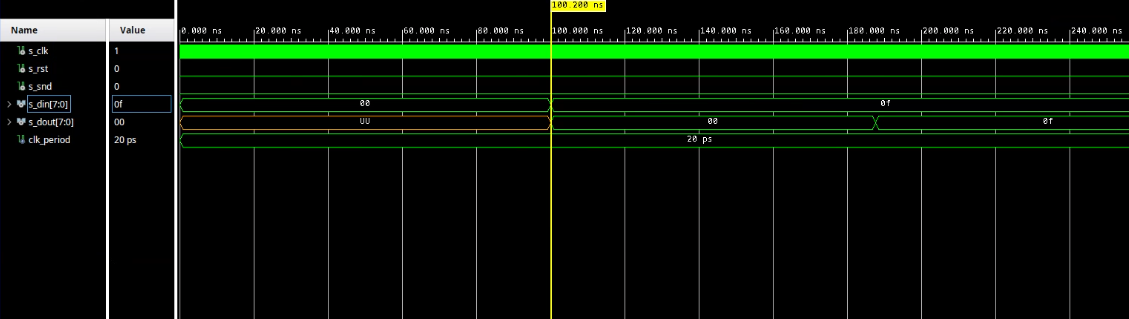
\includegraphics[width=17cm]{immagini/esercizio9/output_simulazione_9.1.png}
    \caption{Simulazione 9.1}
    \label{fig:my_label}
\end{figure}

\subsection{Sintesi su scheda}
Per implementare il sistema sulla scheda sono stati innanzitutto utilizzati i componenti \textit{button\_debouncer} per gestire gli input dei pulsanti. L'uscita del sistema AB è stata mappata con i led appropriati tramite il file dei constraint.
La modifica principale che è stata apportata riguarda la modifica del clock, che ha particolare incidenza sulla periferica seriale.
La UART è stata infatti impostata con \textit{baud rate} e \textit{baud divide} relativi a una frequenza di 48Mhz, mentre il clock di base della scheda ha una frequenza di 100Mhz. 
È stato quindi inserito un divisore di frequenza che la dimezza in output, e fornisce il clock agli altri componenti del sistema.
Nel file video 9.1 è mostrato il funzionamento della scheda, con diverse trasmissioni e reset.

Di seguito è mostrato il codice relativo al componente che ingloba gli altri:

\begin{lstlisting} [language=VHDL, caption=Testing sistema AB]
library IEEE;
use IEEE.STD_LOGIC_1164.ALL;

entity top is
    Port (
        snd, clk, rst: in std_logic;
        din : in std_logic_vector(7 downto 0);
        dout : out std_logic_vector(7 downto 0)
    );

end top;

architecture Behavioral of top is
    component ab is
        Port (
            snd, clk, rst: in std_logic;
            din : in std_logic_vector(7 downto 0);
            dout : out std_logic_vector(7 downto 0)
        );
    end component ab;

    component ButtonDebouncer is
        generic (
            CLK_period: integer := 10;  -- periodo del clock in nanosec
            btn_noise_time: integer := 10000000 --durata dell'oscillazione in nanosec
        );
        Port ( RST : in STD_LOGIC;
             CLK : in STD_LOGIC;
             BTN : in STD_LOGIC;
             CLEARED_BTN : out STD_LOGIC);
    end component ButtonDebouncer;

    component clock_divider is
        generic(
            clock_frequency_in : integer := 100000000;--100MHz
            clock_frequency_out : integer := 50000000 --50MHz
        );
        Port ( clock_in : in STD_LOGIC;
             reset : in STD_LOGIC;
             clock_out : out STD_LOGIC);
    end component;

    signal db1_out,s_clk: std_logic ;

begin

    db1: ButtonDebouncer port map(
            RST => rst,
            CLK => s_clk ,
            BTN => snd,
            CLEARED_BTN => db1_out

        );

    sis_ab: ab port map(
            snd =>db1_out,
            clk => s_clk,
            rst => rst,
            din => din,
            dout => dout
        );

    divisore: clock_divider
        port map(
            clock_in=>clk ,
            reset=>rst,
            clock_out=>s_clk
        );
end Behavioral;
\end{lstlisting}

















\section{UART MEM}
\paragraph{Traccia} Come variante dell’esercizio 9.1, il sistema A invia al sistema B tramite l’interfaccia seriale N stringhe di 8 bit contenute all’interno di una memoria ROM. Le stringhe ricevute vengono memorizzate in una memoria locale a B. Il progetto deve prevedere che A utilizzi un componente contatore per scandire le N stringhe da inviare.

\subsection{Architettura}
Analogamente all'esercizio precedente il sistema è realizzato con un approccio strutturale. Sono stati aggiunti una serie di componenti per implementare le nuove funzionalità.

Il sistema A è composto da:
\begin{itemize}
    \item \textit{UART}: il componente, fornitoci a priori, costituisce in un'interfaccia per la trasmissione del dato tra i due sistemi;
    \item \textit{rom}: una memoria 4x8 contenente le stringhe da inviare a B;
    \item \textit{contatore}: conta il numero di trasmissioni dei dati, in modo tale da terminare opportunamente lo scambio di messaggi; 
    \item \textit{rete di controllo}: regola che la trasmissione dei dati avvenga in modo corretto.
\end{itemize}

Il sistema B, invece, è composto da:
\begin{itemize}
    \item \textit{UART}: il componente, fornitoci a priori, costituisce in un'interfaccia per la trasmissione del dato tra i due sistemi;
    \item \textit{contatore}: conta il numero di ricezioni dei dati, in modo tale da terminare opportunamente lo scambio di messaggi;
    \item \textit{registro}: registro in cui si è scelto di memorizzare temporaneamente la stringa trasmessa da A;
    \item \textit{memoria}: memoria interna a B, dove vengono memorizzate le stringhe ricevute da A;
    \item \textit{rete di controllo}: regola che la trasmissione e l'output dei dati avvenga in modo corretto.
\end{itemize}

Le interconnessioni tra i due sistemi sono visibili nella seguente architettura: 
\begin{figure}[H]
    \centering
    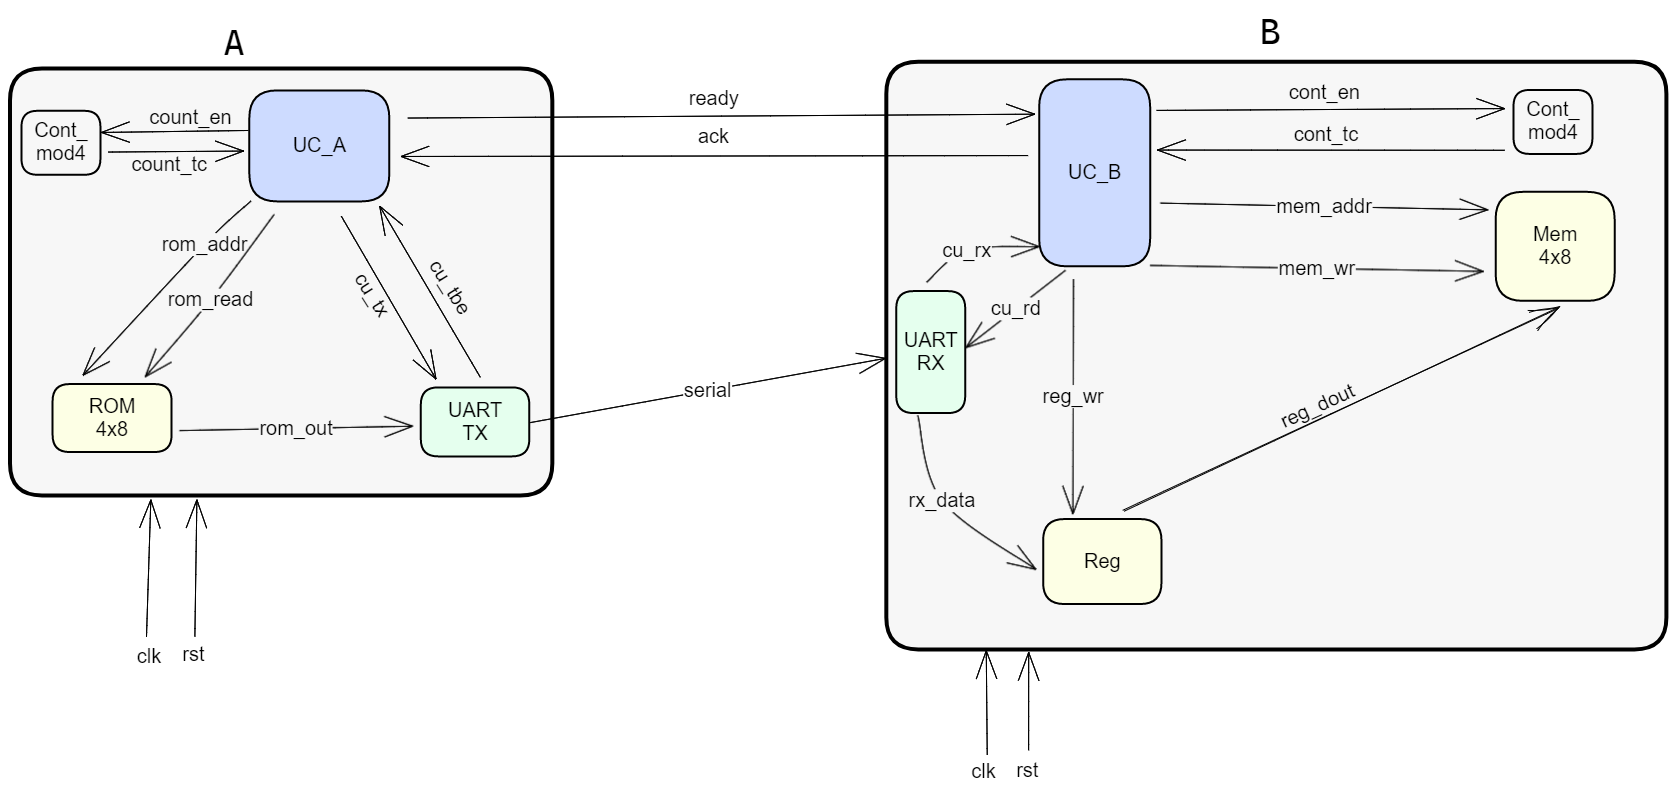
\includegraphics[width=17cm]{immagini/esercizio9/schema_9.2.png}
    \caption{Schema Interfaccia Seriale}
    \label{fig:my_label}
\end{figure}

Gli automi di A e B si occupano di gestire i componenti delle architetture e comunicano tra loro con un semplice \textit{two-way handshake}, con i segnali ready ed ack come descritto nei capitoli precedenti. 
Le differenze principali rispetto all'esercizio precedente stanno nell'assenza del segnale \textit{done}, che indicava ad A la fine della trasmissione, e la necessita di scrivere o leggere dalle memorie interne dei dispositivi incrementando mano mano l'indirizzo.

Nell'automa A oltre al normale autociclo che deve aspettare l'ack alto prima di trasmettere sono stati aggiunti altre due condizioni di \textit{wait} per sincronizzare la comunicazione:
la prima aspetta che il segnale della UART \textit{tbe} sia alto , che indica la fine dell'invio dei dati, e la seconda aspetta che l'ack di B si abbassi, in modo da essere sicuri di non finire e ritrovarlo ancora alto mentre B sta finendo di ricevere, facendo partire una trasmissione errata. La gestione dell'indirizzo per scrivere in memoria e il contatore per scandire il numero di trasmissioni è omologa a quella vista nell'esercizio 7, per cui arrivati al numero massimo si arriverà nello stato idle.

L'automa B ha subito meno variazioni rispetto ad A, ci sono due auto-cicli per aspettare il segnale di \textit{ready} alto e per aspettare il segnale \textit{RDA} della UART, in modo da poter alzare il segnale di lettura dalla seriale, scrivere il valore in un registro temporaneo, e poi scrivere in memoria il risultato alla locazione giusta.
L'utilizzo del registro temporaneo permette ai componenti delle seriali di riprendere il prima possibile la comunicazione senza impattare sul dato già arrivato, che in contemporanea sta venendo scritto in memoria. Se l'uscita del ricevitore fosse stata collegata direttamente alla memoria ci sarebbe stato il rischio di un cambio del dato.

Di seguito è possibile osservare la stesura degli automi dei singoli sistemi: 
\begin{figure}[H]
    \centering
    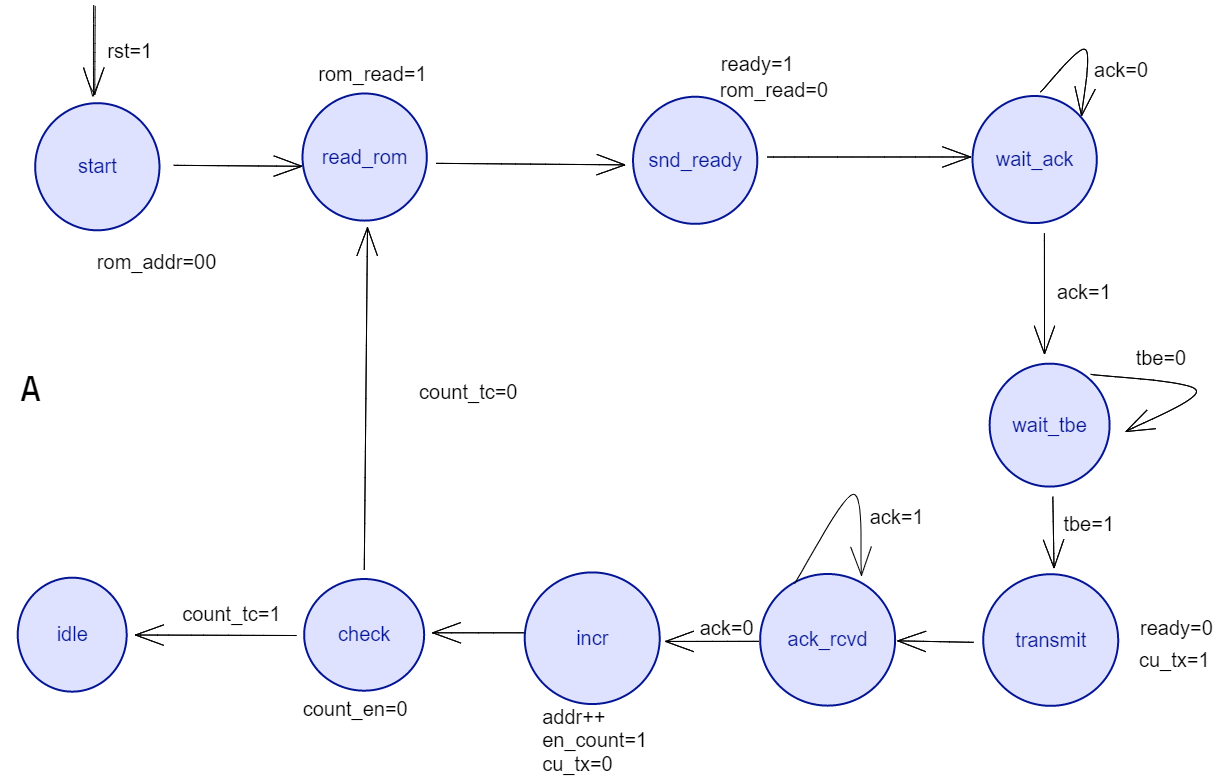
\includegraphics[width=17cm]{immagini/esercizio9/automaA_9.2.png}
    \caption{Automa A}
    \label{fig:my_label}
\end{figure}

\begin{figure}[H]
    \centering
    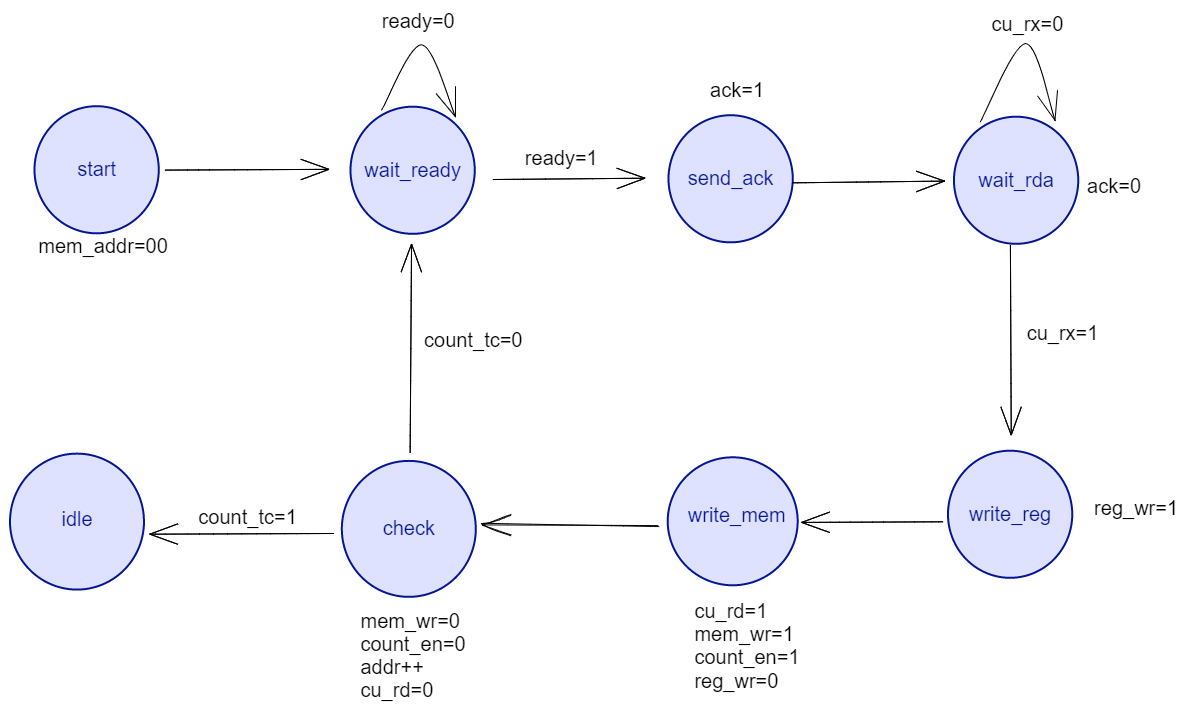
\includegraphics[width=17cm]{immagini/esercizio9/automaB_9.2.png}
    \caption{Automa B}
    \label{fig:my_label}
\end{figure}


Di seguito il codice di A e B:
N.B.: per semplicità è stato omesso il codice della UART.
\begin{lstlisting} [language=VHDL, caption=Contatore mod4]
library IEEE;
use IEEE.std_logic_1164.all;
use IEEE.numeric_std.all;

entity cont_mod4 is
    port (
        clk, rst: in std_logic;
        tc: out std_logic
    );
end entity cont_mod4;

architecture rtl of cont_mod4 is
    signal count: std_logic_vector(1 downto 0) := "00";
begin
    cont: process(clk)
    begin
        if rising_edge(clk) then
            if rst = '1' then
                count <="00";
                tc <= '0';
            elsif count = "11" then
                tc <= '1';
                count <= (others => '0');
            else 
                 tc <= '0';
                 count <= std_logic_vector((unsigned(count) + 1));
               
            end if;
        end if;
   end process cont;
    
end architecture rtl;
\end{lstlisting}

\begin{lstlisting} [language=VHDL, caption=Rete di controllo di A]
library IEEE;
use IEEE.STD_LOGIC_1164.ALL;
use IEEE.numeric_std.all;

entity cu_a is
    port(
        clk, rst, ack, count_tc, cu_tbe: in std_logic;
        ready, cu_tx, rom_read, count_en: out std_logic;
        rom_addr: out std_logic_vector(1 downto 0)
    );
end cu_a;

architecture behavioral of cu_a is

    type state is (
        START,
        READ_ROM,
        SND_READY,
        WAIT_ACK,
        WAIT_TBE,
        TRANSMIT,
        ACK_RCVD,
        INCR,   
        CHECK,
        IDLE
    );
    signal current_state : state:= IDLE;
    signal next_state : state;
    signal s_addr: std_logic_vector(1 downto 0) := "00";

begin
    comb: process(current_state, ack, cu_tbe)
    begin
        case current_state is

            when START =>
                ready <= '0';
                s_addr <= "00";
                rom_read <= '0';
                cu_tx <= '0';
                count_en <= '0';
                next_state<= READ_ROM;

            when READ_ROM=>
                rom_read <= '1';
                next_state <= SND_READY;

            when SND_READY=>
                rom_read <= '0';
                ready <= '1';
                next_state <= WAIT_ACK;

            when WAIT_ACK=>
                if ( ack = '1' ) then
                    next_state <= WAIT_TBE;
                else
                    next_state <= WAIT_ACK;
                end if;

            when WAIT_TBE =>
                if cu_tbe = '1' then
                    next_state <= TRANSMIT;
                else
                    next_state <= WAIT_TBE;
                end if;

            when TRANSMIT=>
                cu_tx <= '1';
                ready <= '0';
                next_state <= ACK_RCVD;
                
            when ACK_RCVD => 
                if ack = '0' then
                    next_state <=  INCR;
                else 
                    next_state <= ACK_RCVD;
                end if;

           when INCR =>
                cu_tx <= '0';
                s_addr <= std_logic_vector((unsigned(s_addr) + 1));
                count_en <= '1';
                next_state <= CHECK;
    
            when CHECK =>
                count_en <= '0';
                if count_tc = '1' then
                    next_state <= IDLE;
                else
                    next_state <= READ_ROM;
                end if;

            when IDLE=>
                next_state<= IDLE;
            when others => next_state<= IDLE;
        end case;
    end process comb;

    rom_addr <= s_addr;

    seq: process(clk)
    begin
        if rising_edge(clk) then
            if rst='1'  then
                current_state<=START;
            else
                current_state<=next_state;
            end if;
        end if;
    end process seq;
end behavioral;
\end{lstlisting}

\begin{lstlisting} [language=VHDL, caption=Rom di A]
library ieee;
use ieee.std_logic_1164.all;
use ieee.numeric_std.all;

entity rom_a is
port(
    clk, read : in std_logic; 
    addr : in std_logic_vector(1 downto 0);
    data : out std_logic_vector(7 downto 0)
    );
end rom_a;

architecture behavioral of rom_a is 
type rom_t is array (0 to 3) of std_logic_vector(7 downto 0);
signal rom : rom_t := (
    "00000010", 
    "00000110", 
    "00001001", 
    "00001111"
);

begin

process(clk)
  begin
    if rising_edge(clk) then
        if read = '1' then
            data <= rom(to_integer(unsigned(addr)));
        end if;
    end if;
end process;
end behavioral;
\end{lstlisting}

Di seguito il codice di A:
\begin{lstlisting} [language=VHDL, caption=Sistema A]
library IEEE;
use IEEE.STD_LOGIC_1164.ALL;

entity a is
    Port (
        clk, ack, rst: in std_logic ;
        ready, data: out std_logic
    );
end a;

architecture Structural of a is

    component cont_mod4 is
        port (
            clk, rst: in std_logic;
            tc: out std_logic
        );
    end component cont_mod4;

    component cu_a is
        port(
            clk, rst, ack, count_tc, cu_tbe: in std_logic;
            ready, cu_tx, rom_read, count_en : out std_logic;
            rom_addr: out std_logic_vector(1 downto 0)
        );
    end component cu_a;


    component rom_a is
        port(
            clk, read : in std_logic;
            addr : in std_logic_vector(1 downto 0);
            data : out std_logic_vector(7 downto 0)
        );
    end component rom_a;

    component UARTcomponent is
        Generic (
            --@48MHz
            --		BAUD_DIVIDE_G : integer := 26; 	--115200 baud
            --		BAUD_RATE_G   : integer := 417

            --@26.6MHz
            BAUD_DIVIDE_G : integer := 14; 	--115200 baud
            BAUD_RATE_G   : integer := 231
        );
        Port (
            TXD 	: out 	std_logic  	:= '1';					-- Transmitted serial data output
            RXD 	: in  	std_logic;							-- Received serial data input
            CLK 	: in  	std_logic;							-- Clock signal
            DBIN 	: in  	std_logic_vector (7 downto 0);		-- Input parallel data to be transmitted
            DBOUT 	: out 	std_logic_vector (7 downto 0);		-- Recevived parallel data output
            RDA		: inout  std_logic;							-- Read Data Available
            TBE		: out 	std_logic 	:= '1';					-- Transfer Buffer Emty
            RD		: in  	std_logic;							-- Read Strobe
            WR		: in  	std_logic;							-- Write Strobe
            PE		: out 	std_logic;							-- Parity error		
            FE		: out 	std_logic;							-- Frame error
            OE		: out 	std_logic;							-- Overwrite error
            RST		: in  	std_logic	:= '0');				-- Reset signal

    end component  UARTcomponent;

    signal count_en, count_tc, rom_read, cu_tx, cu_tbe: std_logic := '0';
    signal rom_addr: std_logic_vector(1 downto 0) := "00";
    signal rom_out: std_logic_vector(7 downto 0) := "00000000";

begin

    cont : cont_mod4
        port map(
            clk=>count_en,
            rst=>rst,
            tc=>count_tc
        );

    cu : cu_a
        port map(
            clk=>clk,
            rst=>rst,
            count_tc=>count_tc ,
            count_en => count_en,
            rom_addr=>rom_addr,
            rom_read=>rom_read,
            ready=>ready,
            ack=>ack,
            cu_tx => cu_tx,
            cu_tbe=>cu_tbe
        );

    rom : rom_a
        port map(
            clk=>clk,
            read=>rom_read,
            addr=>rom_addr,
            data=>rom_out
        );

    uart:  UARTcomponent generic map(
            BAUD_DIVIDE_G=>26,
            BAUD_RATE_G=>417
        )
        port map (
            TXD => data,
            RXD => '1',
            CLK => clk,
            DBIN => rom_out,
            DBOUT => OPEN,
            RDA => OPEN,
            TBE => cu_tbe,
            RD => '0',
            WR => cu_tx,
            PE => OPEN,
            FE => OPEN,
            OE => OPEN,
            RST => rst
        );

end Structural;

\end{lstlisting}


N.B.: il codice del contatore mod4 coincide con il codice del contatore del sistema A e per semplicità è stato omesso il codice della UART.
\begin{lstlisting} [language=VHDL, caption=Registro di B]
library IEEE;
use IEEE.STD_LOGIC_1164.ALL;

entity reg is
    port (
        d: in std_logic_vector (7 downto 0);
        clk, rst: in std_logic ;
        write: in std_logic ;
        q:out std_logic_vector (7 downto 0));
end reg;

architecture Behavioral of reg is

begin
    process (clk)
    begin
        if rising_edge (clk) then
            if (rst='1') then
                q<="00000000";
            elsif(write='1') then
                q<=d;
            end if;
        end if;
    end process;

end Behavioral;

\end{lstlisting}

\begin{lstlisting} [language=VHDL, caption=Memoria di B]
library ieee;
use ieee.std_logic_1164.all;
use ieee.numeric_std.all;

entity memory is
    port(
        clk, write, rst : in std_logic;
        addr : in std_logic_vector(1 downto 0);
        input : in std_logic_vector(7 downto 0);
        output : out std_logic_vector(7 downto 0)
    );
end memory;

architecture behavioral of memory is
    type mem_t is array (0 to 3) of std_logic_vector(7 downto 0);
    signal mem : mem_t := (
        "00000000",
        "00000000",
        "00000000",
        "00000000"
    );

begin
    process(clk)
    begin
        if rising_edge(clk) then
            if rst = '1' then
                for i in 0 to 3 loop
                    mem(i) <= "00000000";
                end loop;
            elsif write = '1' then
                mem(to_integer(unsigned(addr))) <= input;
            end if;
        end if;
        output<=mem(to_integer(unsigned(addr)));
    end process;
end behavioral;
\end{lstlisting}

\begin{lstlisting} [language=VHDL, caption=Rete di controllo di B]
library IEEE;
use IEEE.STD_LOGIC_1164.ALL;
use IEEE.numeric_std.all;

entity cu_b is
    port(
        clk, rst, ready,  count_tc, cu_rx: in std_logic;
        ack, count_en, reg_wr, mem_wr, cu_rd: out std_logic;
        mem_addr: out std_logic_vector(1 downto 0)
    );
end cu_b;

architecture behavioral of cu_b is

    type state is (
        START,
        WAIT_READY,
        SEND_ACK,
        WAIT_RDA,
        WRITE_REG,
        WRITE_MEM,
        CHECK,
        IDLE
    );
    signal current_state : state:= IDLE;
    signal next_state : state;
    signal s_addr: std_logic_vector(1 downto 0) :=(others => '0');

begin
    comb: process(current_state, ready, cu_rx)
        variable somma: unsigned(8 downto 0) := (others => '0');
    begin
        case current_state is

            when START =>
                ack <= '0';
                s_addr <= "00";
                count_en <= '0';
                cu_rd <= '0';
                mem_wr <= '0';
                reg_wr <= '0';
                next_state<= WAIT_READY;

            when WAIT_READY=>
                if ( ready = '1' ) then
                    next_state <= SEND_ACK;
                else
                    next_state <= WAIT_READY;
                end if;

            when SEND_ACK=>
                ack <= '1';
                next_state <= WAIT_RDA;

            when WAIT_RDA=>
                ack <= '0';
                if ( cu_rx = '1' ) then
                    next_state <= WRITE_REG;
                else
                    next_state <= WAIT_RDA;
                end if;

            when WRITE_REG=>
                reg_wr <= '1';
                next_state <= WRITE_MEM;

            when WRITE_MEM=>
                cu_rd <= '1';
                mem_wr <= '1';
                count_en <= '1';
                reg_wr <= '0';
                next_state <= CHECK;

            when CHECK =>
                mem_wr <= '0';
                cu_rd <= '0';
                count_en <= '0';
                s_addr <= std_logic_vector((unsigned(s_addr) + 1));
                
                if count_tc = '1' then
                    next_state <= IDLE;
                else
                    next_state <= WAIT_READY;
                end if;

            when IDLE=>
                next_state<= IDLE;
            when others => next_state<= IDLE;
        end case;
    end process comb;

    mem_addr <= s_addr;

    seq: process(clk)
    begin
        if rising_edge(clk) then
            if rst='1'  then
                current_state<=START;
            else
                current_state<=next_state;
            end if;
        end if;
    end process seq;
end behavioral;
\end{lstlisting}

\begin{lstlisting} [language=VHDL, caption=Sistema B]
library IEEE;
use IEEE.STD_LOGIC_1164.ALL;

entity b is
    Port (
        clk, ready, rst, serial_in: in std_logic ;
        ack: out std_logic
    );
end b;

architecture Structural of b is

    component cont_mod4 is
        port (
            clk, rst: in std_logic;
            tc: out std_logic
        );
    end component cont_mod4;

    component reg is
        port (
            d: in std_logic_vector (7 downto 0);
            clk, rst: in std_logic ;
            write: in std_logic ;
            q:out std_logic_vector (7 downto 0));
    end component reg;

    component cu_b is
        port(
            clk, rst, ready,  count_tc, cu_rx: in std_logic;
            ack, count_en, reg_wr, mem_wr, cu_rd: out std_logic;
            mem_addr: out std_logic_vector(1 downto 0)
        );
    end component cu_b;

    component memory is
        port(
            clk, write, rst : in std_logic;
            addr : in std_logic_vector(1 downto 0);
            input : in std_logic_vector(7 downto 0);
            output : out std_logic_vector(7 downto 0)
        );
    end  component memory;

    component UARTcomponent is
        Generic (
            --@48MHz
            --		BAUD_DIVIDE_G : integer := 26; 	--115200 baud
            --		BAUD_RATE_G   : integer := 417

            --@26.6MHz
            BAUD_DIVIDE_G : integer := 14; 	--115200 baud
            BAUD_RATE_G   : integer := 231
        );
        Port (
            TXD 	: out 	std_logic  	:= '1';					-- Transmitted serial data output
            RXD 	: in  	std_logic;							-- Received serial data input
            CLK 	: in  	std_logic;							-- Clock signal
            DBIN 	: in  	std_logic_vector (7 downto 0);		-- Input parallel data to be transmitted
            DBOUT 	: out 	std_logic_vector (7 downto 0);		-- Recevived parallel data output
            RDA		: inout  std_logic;							-- Read Data Available
            TBE		: out 	std_logic 	:= '1';					-- Transfer Buffer Emty
            RD		: in  	std_logic;							-- Read Strobe
            WR		: in  	std_logic;							-- Write Strobe
            PE		: out 	std_logic;							-- Parity error		
            FE		: out 	std_logic;							-- Frame error
            OE		: out 	std_logic;							-- Overwrite error
            RST		: in  	std_logic	:= '0');				-- Reset signal

    end component  UARTcomponent;

    signal count_en, count_tc, cu_rx, cu_rd, mem_wr, reg_wr: std_logic := '0';
    signal mem_addr: std_logic_vector(1 downto 0) := "00";
    signal rx_data, reg_dout: std_logic_vector(7 downto 0) := "00000000";

begin

    cont : cont_mod4
        port map(
            clk=>count_en,
            rst=>rst,
            tc=>count_tc
        );

    reg_b: reg
        port map(
            clk=> clk,
            rst=>rst,
            write=>reg_wr,
            d=>rx_data,
            q=>reg_dout
        );

    cu : cu_b
        port map(
            clk=>clk,
            rst=>rst,
            count_tc=>count_tc ,
            count_en => count_en,
            mem_addr=>mem_addr,
            mem_wr => mem_wr,
            reg_wr => reg_wr,
            ready=>ready,
            ack=>ack,
            cu_rx => cu_rx,
            cu_rd => cu_rd
        );


    mem: memory 
        port map(
            clk=>clk,
            rst=>rst,
            write => mem_wr,
            addr=>mem_addr,
            input=>reg_dout,
            output=>OPEN
        );
 
    uart:  UARTcomponent generic map(
            BAUD_DIVIDE_G=>26,
            BAUD_RATE_G=>417
        )
        port map (
            TXD => OPEN,
            RXD => serial_in,
            CLK => clk,
            DBIN => "00000000",
            DBOUT => rx_data,
            RDA => cu_rx,
            TBE => OPEN,
            RD => cu_rd,
            WR => '0',
            PE => OPEN,
            FE => OPEN,
            OE => OPEN,
            RST => rst
        );

end Structural;

\end{lstlisting}

Infine, è possibile osservare il codice dell'intero sistema AB:
\begin{lstlisting} [language=VHDL, caption=Sistema AB]
library IEEE;
use IEEE.STD_LOGIC_1164.ALL;

entity ab is
 Port (
    clk, rst: in std_logic
  );
end ab;

architecture Structural of ab is

component a is
    Port (
        clk, ack, rst: in std_logic ;
        ready, data: out std_logic
    );
end component a;

component b is
    Port (
        clk, ready, rst, serial_in: in std_logic ;
        ack: out std_logic
    );
end component b;

signal ack, ready, data: std_logic := '0';

begin
    UnitA: a port map(
        clk=>clk,
        rst=>rst,
        ready=>ready,
        ack=>ack,
        data=>data
       );

    UnitB: b port map(
        clk=>clk,
        rst=>rst,
        ready=>ready,
        ack=>ack,
        serial_in=>data
       );


end Structural;

\end{lstlisting}

\subsection{Simulazione}
Per una maggiore sicurezza si è scelto di testare prima la rete di controllo del sistema A singolarmente e poi di effettuare la simulazione dell'intero sistema di Interfaccia Seriale.

\begin{figure}[H]
    \centering
    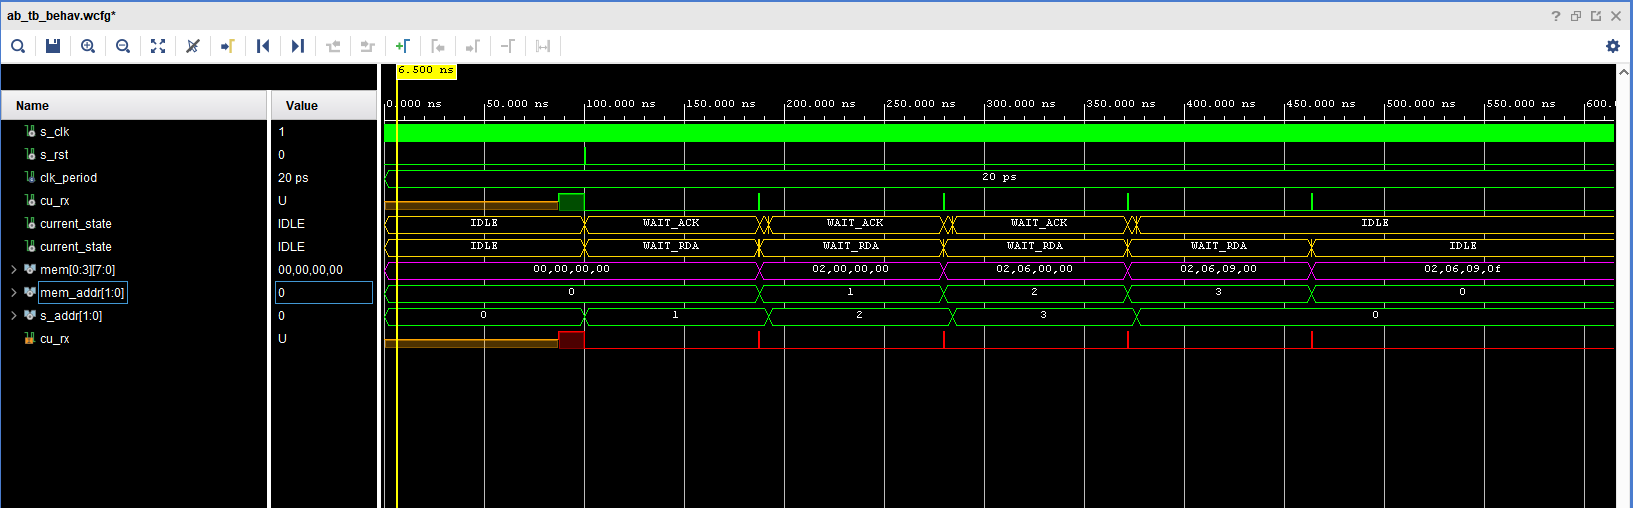
\includegraphics[width=17cm]{immagini/esercizio9/simulazione_9.2.png}
    \caption{Simulazione AB}
    \label{fig:sim_9.2}
\end{figure}


\paragraph{Testbench}

\begin{lstlisting} [language=VHDL, caption=Testing rete di controllo di A]
library IEEE;
use IEEE.STD_LOGIC_1164.ALL;

entity cu_a_tb is
end cu_a_tb;

architecture Behavioral of cu_a_tb is

    component cu_a is
        port(
            clk, rst, ack, done, count_tc: in std_logic;
            ready, cu_tx, rom_read, count_en : out std_logic;
            rom_addr: out std_logic_vector(1 downto 0)
        );
    end component cu_a;

    signal s_clk, s_rst, s_count_tc, s_count_en, s_ready, s_done, s_ack, s_cu_tx, s_rom_read: std_logic := '0';
    signal s_rom_addr : std_logic_vector(1 downto 0) := "00";
    constant clk_period:time := 10ns;

begin

    uut : cu_a
        port map(
            clk=>s_clk,
            rst=>s_rst,
            count_tc=>s_count_tc ,
            count_en => s_count_en,
            rom_addr=>s_rom_addr,
            rom_read=>s_rom_read,
            ready=>s_ready,
            done => s_done,
            ack=>s_ack,
            cu_tx => s_cu_tx
        );

    tb: process
    begin
        wait for 100ns;
        s_rst <='1';
        wait for clk_period;
        s_rst <='0';

        wait until s_ready = '1';
        wait for clk_period;
        s_ack <= '1';
        wait for clk_period;
        s_ack <= '0';
        wait for clk_period;
        s_done <= '1';
        wait for clk_period;
        s_done <= '0';
        wait for clk_period;
    
        wait;
    end process tb;

    clock: process
    begin
        loop
            s_clk <= not s_clk;
            wait for clk_period/2;
        end loop;
    end process clock;

end Behavioral;

\end{lstlisting}

\begin{lstlisting} [language=VHDL, caption=Testing sistema AB]
library IEEE;
use IEEE.STD_LOGIC_1164.ALL;

entity ab_tb is
end ab_tb;

architecture Behavioral of ab_tb is

   component ab is port (         
        clk,rst: in std_logic        
  );
    end component ab;

    signal s_clk, s_rst: std_logic := '0';
    constant clk_period: time := 20ps;

begin
    uut: AB port map(
            clk=>s_clk,         
            rst=>s_rst
        );

    tb: process
    begin
        wait for 100ns;
        s_rst <='1';
        wait for clk_period;
        s_rst <='0';
        
        wait;
    end process tb;

    clock: process
    begin
        loop
            s_clk <= not s_clk;
            wait for clk_period/2;
        end loop;
    end process clock;
end Behavioral;
\end{lstlisting}

